\documentclass[a4paper,12pt]{article}
%%%%%%%%%%%%%%%%%%%%%%%%%%%%%%%%%%%%%%%%%%%%%%%%%%%%%%%%%%%%%%%%%%%%%%%%%%%%%%%%%%%%%%%%%%%%%%%%%%%%%%%%%%%%%%%%%%%%%%%%%%%%%%%%%%%%%%%%%%%%%%%%%%%%%%%%%%%%%%%%%%%%%%%%%%%%%%%%%%%%%%%%%%%%%%%%%%%%%%%%%%%%%%%%%%%%%%%%%%%%%%%%%%%%%%%%%%%%%%%%%%%%%%%%%%%%
\usepackage{eurosym}
\usepackage{vmargin}
\usepackage{amsmath}
\usepackage{graphics}
\usepackage{epsfig}
\usepackage{subfigure}
\usepackage{fancyhdr}
%\usepackage{listings}
\usepackage{framed}
\usepackage{graphicx}

\setcounter{MaxMatrixCols}{10}
%TCIDATA{OutputFilter=LATEX.DLL}
%TCIDATA{Version=5.00.0.2570}
%TCIDATA{<META NAME="SaveForMode" CONTENT="1">}
%TCIDATA{LastRevised=Wednesday, February 23, 2011 13:24:34}
%TCIDATA{<META NAME="GraphicsSave" CONTENT="32">}
%TCIDATA{Language=American English}

\pagestyle{fancy}
\setmarginsrb{20mm}{0mm}{20mm}{25mm}{12mm}{11mm}{0mm}{11mm}
\lhead{MA4128} \rhead{Mr. Kevin O'Brien}
\chead{Advanced Data Modelling}
%\input{tcilatex}


% http://www.norusis.com/pdf/SPC_v13.pdf
\begin{document}


%SESSION 1: Hierarchical Clustering
% Hierarchical clustering - dendrograms
% Divisive vs. agglomerative methods
% Different linkage methods

%SESSION 2: K-means Clustering

\tableofcontents
\newpage

 \section{Review of Last Class}
 \begin{itemize}
 	\item Cluster analysis is a convenient method for identifying homogenous groups of
 	objects called clusters. Objects (or cases, observations) in a specific cluster share
 	many characteristics, but are very dissimilar to objects not belonging to that cluster.
 	\item  There are three cluster analysis approaches: hierarchical methods,
 	partitioning methods (more precisely, k-means), and two-step clustering,
 	which is largely a combination of the first two methods. In the last class we looked as hierarchical clustering analysis.
 	\item Each of these procedures
 	follows a different approach to grouping the most similar objects into a cluster and
 	to determining each object�s cluster membership.
 	\item Some approaches � most notably hierarchical methods � require us to specify how similar or different objects
 	are in order to identify different clusters. Most software packages, such as SPSS, calculate a measure
 	of (dis)similarity by estimating the distance between pairs of objects. Objects with
 	smaller distances between one another are more similar, whereas objects with larger
 	distances are more dissimilar.
 	\item An important problem in the application of cluster analysis is the decision
 	regarding how many clusters should be derived from the data. This question is
 	explored in the next step of the analysis. Sometimes, however,
 	number of segments that have to be derived from the data will be known in advance.
 	\item
 	By choosing a specific clustering procedure, we determine how clusters are to be
 	formed. (This always involves optimizing some kind of criterion, such as minimizing
 	the within-cluster variance (i.e., the clustering variables� overall variance of
 	objects in a specific cluster), or maximizing the distance between the objects or
 	clusters). The procedure could also address the question of how to determine the
 	(dis)similarity between objects in a newly formed cluster and the remaining objects
 	in the dataset.
 	\item
 	Hierarchical clustering procedures are characterized by the tree-like structure
 	established in the course of the analysis. Most hierarchical techniques fall into a
 	category called agglomerative clustering. In this category, clusters are consecutively
 	formed from objects. Initially, this type of procedure starts with each object
 	representing an individual cluster. These clusters are then sequentially merged
 	according to their similarity. First, the two most similar clusters (i.e., those with
 	the smallest distance between them) are merged to form a new cluster at the bottom
 	of the hierarchy. In the next step, another pair of clusters is merged and linked to a
 	higher level of the hierarchy, and so on. This allows a hierarchy of clusters to be
 	established from the bottom up.
 	\item A cluster hierarchy can also be generated top-down. In this divisive clustering,
 	all objects are initially merged into a single cluster, which is then gradually split up. Divisive procedures are quite rarely used in practice. We therefore
 	concentrate on the agglomerative clustering procedures.
 	\item This means that if an object is assigned
 	to a certain cluster, there is no possibility of reassigning this object to another
 	cluster. This is an important distinction between these types of clustering and
 	partitioning methods such as \textbf{\textit{k-means}}.
 	\newpage
 	\item
 	In statistics, the occurrence of several  variables in a multiple regression model are \textbf{closely correlated} to one another, and carrying the same information, more or less. Multi-collinearity can cause strange results when attempting to study how well individual independent variables contribute to an understanding of the dependent variable, often undermining the analysis.
 	
 	\item In many analysis tasks, the variables under consideration are measured on
 	different scales or levels. This would
 	clearly distort any clustering analysis results. We can resolve this problem by \textbf{\textit{standardizing}}
 	the data prior to the analysis.
 	
 	\item Different standardization methods are available, such as the simple \textbf{\textit{z standardization}},
 	which re-scales each variable to have a mean of 0 and a standard deviation of 1.
 	
 	\item In most situations, however, \textbf{\textit{standardization by range}}(e.g., to a
 	range of 0 to 1 or -1 to 1) is preferable. We recommend standardizing the data
 	in general, even though this procedure can potentially reduce or inflate the variables� influence
 	on the clustering solution.
 	
 	
 	
 	An understanding of linkage method's other than than Ward method will be expected in the end of year examination.
 	
 	\item A common way to visualize the cluster analysis�s progress is by drawing a
 	dendrogram, which displays the distance level at which there was a combination
 	of objects and clusters.
 	Here is an example of a dendrogram (which corresponds to the example in the next section of material.
 	
 	
 	\begin{figure}[h!]
 		\begin{center}
 			% Requires \usepackage{graphicx}
 			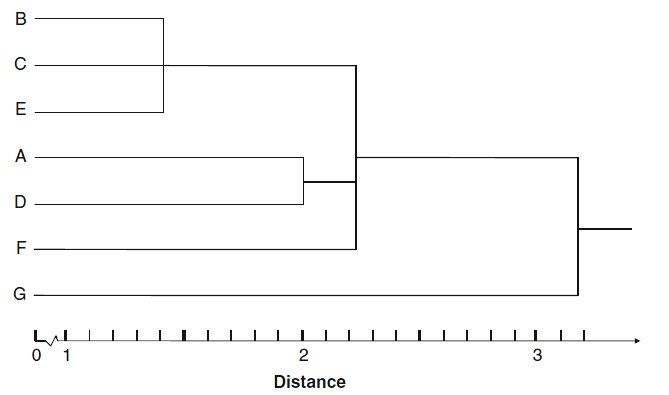
\includegraphics[scale=0.6]{images/Dendrogram.jpg}\\
 		\end{center}
 	\end{figure}
 	
 	\item An important question is how to decide on the number of
 	clusters to retain from the data. Unfortunately, hierarchical methods provide only
 	very limited guidance for making this decision. The only meaningful indicator
 	relates to the distances at which the objects are combined. Similar to factor
 	analysis�s scree plot, we can seek a solution in which an additional combination
 	of clusters or objects would occur at a greatly increased distance. This raises the
 	issue of what a great distance is, of course. For this purpose, we can make use of the dendrogram.
 	
 	\item In constructing the dendrogram, SPSS rescales the distances to a range
 	of 0�25; that is, the last merging step to a one-cluster solution takes place at a
 	(rescaled) distance of 25. The rescaling often lengthens the merging steps, thus
 	making breaks occurring at a greatly increased distance level more obvious.
 	Despite this, this distance-based decision rule does not work very well in all
 	cases.
 	
 	It is often difficult to identify where the break actually occurs. This is also
 	the case in our example above. By looking at the dendrogram, we could justify
 	a two-cluster solution ([A,B,C,D,E,F] and [G]), as well as a five-cluster solution
 	([B,C,E], [A], [D], [F], [G]).
 	
 	
 \end{itemize}
 \newpage
\section{Introduction to Cluster Analysis}


%Introduction
\begin{itemize}
\item \textbf{\textit{A cluster is a group of relatively homogeneous cases or observations.}}
\item Cluster analysis is a major technique for classifying a large volumes of information into
manageable meaningful piles. Cluster analysis is a data reduction tool that creates subgroups that are
more manageable than individual data items. 
\item The term cluster analysis encompasses a number of different algorithms and methods for grouping objects of similar kind into respective categories.A general question facing researchers in many areas of inquiry is how to organize observed data into meaningful structures, that is, to develop \textbf{\emph{taxonomies}}.

\item In other words cluster analysis is an exploratory data analysis tool which aims at sorting different objects into groups in a way that the degree of association between two objects is maximal if they belong to the same group and minimal otherwise. Given the above, cluster analysis can be used to discover structures in data without providing an explanation/interpretation. 
\item In other words, cluster analysis simply discovers structures in data without explaining why they exist. Like factor analysis, it examines the full complement
of inter-relationships between variables. Both cluster analysis (and later, discriminant
analysis) are concerned with classification.

\item However, the latter requires prior knowledge of membership of each cluster in order to classify new cases. In cluster analysis
there is no prior knowledge about which elements belong to which clusters. 
\item The grouping
or clusters are defined through an analysis of the data. Subsequent multivariate analyses
can be performed on the clusters as groups.
\end{itemize}




\subsection{Types of Cluster Analysis}
There are three main types of cluster analysis.
\begin{itemize}
	\item Hierarchical Clustering Analysis
	\item Non-hierarchical Clustering Analysis (K-means clustering)
	\item Two Step Clustering Analysis
\end{itemize}

Within hierarchical clustering analysis there are two subcategories: 
\begin{itemize}
	\item Agglomerative (start from n clusters,to get to 1 cluster)
	\item Divisive (start from 1 cluster, to get to $n$ cluster)
\end{itemize}
%------------------------------------------------------------------------------%
Cluster analysis is a tool of discovery revealing associations and structure in data which, though not previously
evident, are sensible and useful when discovered. Importantly, CA enables new
cases to be assigned to classes for identification and diagnostic purposes; or find \textbf{\textit{exemplars}}
to represent classes.
%------------------------------------------------------------------------------%
\subsection{Types of Cluster Analysis}
There are three main types of cluster analysis.
\begin{itemize}
	\item Hierarchical Clustering Analysis
	\item Non-hierarchical Clustering Analysis (K-means clustering)
	\item Two Step Clustering Analysis
\end{itemize}
%------------------------------------------------------------------------------%
Within hierarchical clustering analysis there are two subcategories: 
\begin{itemize}
	\item Agglomerative (start from n clusters,to get to 1 cluster)
	\item Divisive (start from 1 cluster, to get to $n$ cluster)
\end{itemize}
%------------------------------------------------------------------------------%


%---------------------------------------------------------------------------------%
\subsection{Statistical Significance Testing}
\begin{itemize}
\item Note that the previous discussions refer to clustering algorithms and do not mention anything about statistical significance testing. 
\item In fact, cluster analysis is not as much a typical statistical test as it is a ``collection" of different algorithms that ``put objects into clusters according to well defined similarity rules."

\item The point here is that, unlike many other statistical procedures, cluster analysis methods are mostly used when we do not have any \textbf{\textit{a priori hypotheses}}, but are still in the exploratory phase of our research. 
\item In a sense, cluster analysis finds the ``most significant solution possible." Therefore, statistical significance testing is really not appropriate here, even in cases when p-values are reported.
\end{itemize}


\section{Simple Case Studies}
\subsection{Applications of Cluster Analysis}

We deal with clustering in almost every aspect of daily life. For example, a group of diners sharing the same table in a restaurant may be regarded as a cluster of people. In food stores items of similar nature, such as different types of meat or vegetables are displayed in the same or nearby locations. There is a countless number of examples in which clustering plays an important role. Clustering techniques have been applied to a wide variety of scientific research problems. For example, in the field of medicine, clustering diseases, cures for diseases, or symptoms of diseases can lead to very useful taxonomies. In the field of psychiatry, the correct diagnosis of clusters of symptoms such as paranoia, schizophrenia, etc. is essential for successful therapy. In archeology, researchers have attempted to establish taxonomies of stone tools, funeral objects, etc. by applying cluster analytic techniques. According to the modern system employed in biology, man belongs to the primates, the mammals, the amniotes, the vertebrates, and the animals.

Note how in this classification, the higher the level of aggregation the less similar are the members in the respective class. Man has more in common with all other primates (e.g., apes) than it does with the more "distant" members of the mammals (e.g., dogs), etc.

In general, whenever we need to classify a "mountain" of information into manageable meaningful piles, cluster analysis is of great utility.


%---------------------------------------------------------------%
\subsection{Market Segmentation}
Suppose a market research company wants to undertake direct mail advertising with specific advertisements
for different groups of people. You could use a variety of independent variabless like \textbf{\textit{family income}}
, \textbf{\textit{age}}, \textbf{\textit{number of cars per family}}, \textbf{\textit{number of mobile phones per family}},\textbf{\textit{number of school children per family}}  etc., to see if different postal or zip codes are characterized by particular combinations of demographic variables which could be grouped together to create a better way of directing the mail out.

This firm might in fact find that postal codes could be grouped into a number of clusters, characterized as ``the retirement zone", ``nappy valley", ``the golf club set", the ``rottweiler in a pick-up" district, etc. This sort of grouping might  be valuable in deciding where to place several new wine stores, or `Tummy to Toddler" shops.

Using cluster analysis, a customer ``type" can represent a homogeneous market segment.
Identifying their particular needs in that market allows products to be designed with greater
precision and direct appeal within the segment. Targeting specific segments is cheaper and
more accurate than broad-scale marketing. Customers respond better to segment marketing
which addresses their specific needs, leading to increased market share and customer
retention.

This is valuable, for example, in banking, insurance and tourism markets. Suppose
four clusters or market segments in the vacation travel industry. They are:
\begin{itemize}
	\item[(1)] The high spending elite - they want top level service and expect to be pampered;
	\item[(2)] The escapists - they want to get away and just relax;
	\item[(3)] The educationalist - they want to see new things, go to museums,
	have a safari, or experience new cultures;
	\item[(4)] the sports person - they want the golf course, tennis court, surfing, deep-sea fishing, climbing, etc.
\end{itemize}
Different brochures and advertising is required for each of these.

Brand image analysis, or defining product `types' by customer perceptions, allows
a company to see where its products are positioned in the market relative to those of its
competitors. This type of modelling is valuable for branding new products or identifying
possible gaps in the market. Clustering supermarket products by linked purchasing patterns
can be used to plan store layouts, maximizing spontaneous purchasing opportunities.

\subsection{A Banking example}
Banking institutions have used hierarchical cluster analysis to develop a typology of customers, for two purposes, as follows:
\begin{itemize}
	\item To retain the loyalty of members by designing the best possible new financial products to meet the needs of different groups (clusters), i.e. new product opportunities.
	\item To capture more market share by identifying which existing services are most profitable for which type of customer and improve market penetration.
\end{itemize}
One major bank completed a cluster analysis on a representative sample of its members, according to 16 variables chosen to reflect the characteristics of their financial transaction patterns. From this analysis, 30 types of members were identified. The results were useful for marketing, enabling the bank to focus on products which had the best financial performance; reduce direct mailing costs and increase response rates by targeting product promotions at those customer types most likely to respond; and consequently, to achieve better branding and customer retention.

This facilitated a differential direct advertising of services
and products to the various clusters that differed inter alia by age, income, risk taking levels, and self-perceived financial needs. In this way, the bank could retain and win the business of more profitable customers at lower costs.

%---------------------------------------------------------------------------------%

\subsection{Steps to conduct a Cluster Analysis}
\begin{enumerate}
	\item Select a distance measure
	\item Select a clustering algorithm
	\item Determine the number of clusters
	\item Validate the analysis
\end{enumerate}
Because we usually don't know the number of groups or clusters that will emerge in our sample and because we want an optimum solution, a two-stage sequence of analysis occurs as follows:

\begin{enumerate}
	\item We carry out a hierarchical cluster analysis using Ward' method applying squared
	\textit{\textbf{Euclidean Distance}} as the distance or similarity measure. This helps to determine the
	optimum number of clusters we should work with.
	\item The next stage is to rerun the hierarchical cluster analysis with our selected number
	of clusters, which enables us to allocate every case in our sample to a particular
	cluster.
\end{enumerate}

%This sequence and methodology using SPSS will be described in more detail later. There are a variety of clustering procedures of which hierarchical cluster analysis is the major one.

\section{Cluster Analysis Techniques}
\begin{itemize}
\item Cluster analysis (CA) is an exploratory data analysis tool for organizing observed data into meaningful taxonomies, groups, or
clusters, based on combinations of independent variables, which maximizes the similarity of cases within
each cluster while maximizing the dissimilarity between groups that are initially unknown.

\item In this sense, CA creates new groupings without any preconceived notion of what clusters
may arise, whereas \textit{\textbf{discriminant analysis}} classifies people and items into
already known groups.

\item Cluster Analysis provides no explanation as to why the clusters exist nor is any
interpretation made. Each cluster thus describes, in terms of the data collected, the class to
which its members belong. Items in each cluster are similar in some ways to each other and
dissimilar to those in other clusters.

\item Cluster analysis is a tool of discovery revealing associations and structure in data which, though not previously
evident, are sensible and useful when discovered. \item Importantly, CA enables new
cases to be assigned to classes for identification and diagnostic purposes; or find \textbf{\textit{exemplars}}
to represent classes.

\end{itemize}

\subsection{Hierarchical cluster analysis}
This is the major statistical method for finding relatively homogeneous clusters of cases based on measured characteristics.

Agglomerative clustering starts with each case as a separate cluster, i.e. there are as many clusters as cases, and then combines the clusters sequentially, reducing the number of clusters at each step until only one cluster is left.

The clustering method uses the dissimilarities or distances between objects when forming the clusters. The SPSS programme calculates \textbf{\textit{distances}} between data points in terms of the specified variables.

A hierarchical tree diagram, called a \textbf{\textit{dendrogram }} on SPSS, can be produced to show the linkage points. The clusters are linked at increasing levels of \textbf{\textit{dissimilarity}}.
The actual measure of dissimilarity depends on the measure used.


\section{Distance measures}
\begin{itemize}
\item 
The joining or tree clustering method uses the dissimilarities (similarities) or distances between objects when forming the clusters. Similarities are a set of rules that serve as criteria for grouping or separating items. 
\item In the previous example the rule for grouping a number of dinners was whether they shared the same table or not. 
\item These distances (similarities) can be based on a single dimension or multiple dimensions, with each dimension representing a rule or condition for grouping objects. For example, if we were to cluster fast foods, we could take into account the number of calories they contain, their price, subjective ratings of taste, etc. The most straightforward way of computing distances between objects in a multi-dimensional space is to compute Euclidean distances. 

\item If we had a two- or three-dimensional space this measure is the actual geometric distance between objects in the space (i.e., as if measured with a ruler). However, the joining algorithm does not "care" whether the distances that are "fed" to it are actual real distances, or some other derived measure of distance that is more meaningful to the researcher; and it is up to the researcher to select the right method for his/her specific application.
Squared Euclidean distance. 

\item You may want to square the standard Euclidean distance in order to place progressively greater weight on objects that are further apart. This distance is computed as (see also the note in the previous paragraph):
\[distance(x,y) = i (xi - yi)^2\]

\end{itemize}

%============================================================================== %




%--------------------------------------------------------------------------------%
\subsection{Distance measures}
Distance can be measured in a variety of ways. There are distances that are Euclidean (can be measured with a ruler) and there are other distances based on similarity. For example, in terms of
geographical distance (i.e. Euclidean distance) Perth, Australia is closer to Jakarta, Indonesia, than it is to Sydney, Australia.

However, if distance is measured in terms of the cities characteristics, Perth is closer to Sydney (e.g. both on a big river estuary, straddling both sides of the river, with surfing beaches, and both English speaking, etc). A number of distance measures are available within SPSS. The \textbf{\textit{squared Euclidean distance}} is the most widely used measure.

\subsection{Euclidean Distance}

The most straightforward and generally accepted way of computing distances between objects in a multi-dimensional space is to compute Euclidean distances, an extension of Pythagoras's theorem.
If we had a two- or three-dimensional space this measure is the actual geometric distance between objects in the space (i.e. as if measured with a ruler).



The Euclidean distance is probably the most commonly chosen type of distance. It simply is the geometric distance in the multidimensional space. The Euclidean distance between two points, x and y, with $k$ dimensions is calculated as:
\[ \sqrt{ \sum^{k}_{j=1} ( x_j - y_j)^2 } \]


In a univariate example, the Euclidean distance between two values is the arithmetic difference, i.e. \textbf{\textit{value1 - value2}}. In the bivariate case, the minimum distance is the hypotenuse of a triangle formed from the points, as in Pythagoras's theorem.
Although difficult to visualize, an extension of the Pythagoras's theorem will give the distance between two points in n-dimensional space. 

The Euclidean distance is always greater than or equal to zero. The measurement would be zero for identical points and high for points that show little similarity.

%======================================================================================= %

\subsection{Euclidean Distance : Worked Example}
Compute the Euclidean Distance between the following points:
$X = \{1,5,4,3\}$ and $Y = \{2,1,8,7\}$

\begin{center}
	\begin{tabular}{|c|c|c|c|}
		\hline
		$x_j$	&	$y_j$	&   $x_j - y_j$	&	$(x_j - y_j)^2$	\\ \hline
		1	&	2	&	-1	&	1	\\
		5	&	1	&	4	&	16	\\
		4	&	8	&	-4	&	16	\\
		3	&	7	&	-4	&	16	\\ \hline
		&		&		&	49	\\ \hline
	\end{tabular}
\end{center}
The Euclidean Distance between the two points is $\sqrt{49}$ i.e. 7.
%--------------------------------------------------------------------------------------%



\subsection{Squared Euclidean distance}


The squared Euclidean distance is used more often than the simple Euclidean distance in order to place progressively greater weight on objects that are further apart. 


The Squared Euclidean distance between two points, x and y, with $k$ dimensions is calculated as:
\[ \sum^{k}_{j=1} ( x_j - y_j)^2  \]
The Squared Euclidean distance may be preferred to the Euclidean distance as it is slightly less computational complex, without loss of any information.

%http://www.econ.upf.edu/~michael/stanford/maeb4.pdf
%http://stn.spotfire.com/spotfire_client_help/hc/hc_distance_measures_overview.htm

%=========================================== %


\subsection{Manhattan (City Block) Distance}
The City-block (Manhattan) distance is simply the average difference across dimensions. In most cases, this distance measure yields results similar to the simple Euclidean distance. However, note that in this measure, the effect of single large differences (outliers) is dampened (since they are not squared). 

%The city-block distance is computed as: distance(x,y) = i |xi - yi|


The City block distance between two points, x and y, with $k$ dimensions is calculated as:
\[ \sum^{k}_{j=1} | x_j - y_j |  \]

The City block distance is always greater than or equal to zero. The measurement would be zero for identical points and high for points that show little similarity.

\subsubsection{Example}
Compute the Manhattan Distance between the following points: 
$X = \{1,3,4,2\}$ and $Y = \{5,2,5,2\}$


\begin{center}
	\begin{tabular}{|c|c|c|c|}
		\hline
		$x_j$	&	$y_j$	&   $x_j - y_j$	&	$| x_j - y_j |$	\\ \hline
		1	&	5	&	-4	&	4	\\
		3	&	2	&	1	&	1	\\
		4	&	5	&	-1	&	1	\\
		2	&	2	&	0	&	0	\\ \hline
		& & & 6 \\
		\hline
	\end{tabular}
\end{center}
The Manhattan Distance between the two points is 6.


%--------------------------------------------------------------------------------%

\begin{itemize}
	\item There are various measures to express (dis)similarity between pairs of objects.
	A straightforward way to assess two objects� proximity is by drawing a straight line
	between them.This type of distance is also referred to as
	\textbf{\textit{Euclidean distance}} (or straight-line distance) and is the most commonly used type
	when it comes to analyzing ratio or interval-scaled data.
	\begin{figure}[h!]
		\begin{center}
			% Requires \usepackage{graphicx}
			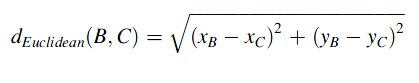
\includegraphics[scale=0.6]{images/EuclidDistance1.jpg}\\
		\end{center}
	\end{figure}
	
	The Euclidean distance is the square root of the sum of the squared differences in
	the variables� values. Suppose B and C were positioned as $(7,6)$ and $(6,5)$ respectively.
	\begin{figure}[h!]
		\begin{center}
			% Requires \usepackage{graphicx}
			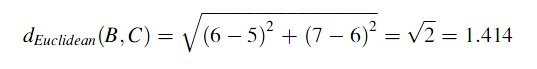
\includegraphics[scale=0.6]{images/EuclidDistance2.jpg}\\
		\end{center}
	\end{figure}
	
	This distance corresponds to the length of the line that connects objects B and C.
	In this case, we only used two variables but we can easily add more under the root
	sign in the formula. However, each additional variable will add a dimension to our
	research problem (e.g., with ten clustering variables, we have to deal with ten
	dimensions), making it impossible to represent the solution graphically.
	
	\item  The \textbf{\textit{Squared Euclidean distance}} uses the same equation as the Euclidean distance metric, but does not take the square root. In the previous example, the squared Euclidean distance between B and C is 2.
	As a result, clustering with the Squared Euclidean distance is computationally faster than clustering with the regular Euclidean distance.
	
	\item We can compute the distance between all other pairs of objects. All
	these distances are usually expressed by means of a \textit{\textbf{distance matrix}}. In this distance
	matrix, the non-diagonal elements express the distances between pairs of objects
	and zeros on the diagonal (the distance from each object to itself is, of course, 0). In
	our example, the distance matrix is an $8 \times 8$ table with the lines and rows
	representing the objects under consideration.
	\begin{figure}[h!]
		\begin{center}
			% Requires \usepackage{graphicx}
			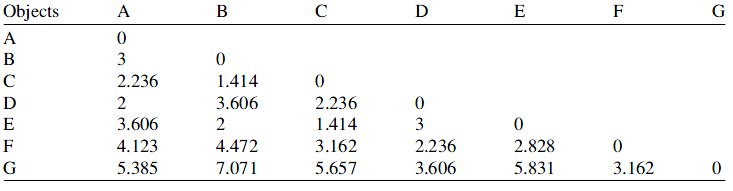
\includegraphics[scale=0.6]{images/DistanceMatrix.jpg}\\
		\end{center}
	\end{figure}
	
	\item There are also alternative distance measures: The \textbf{\textit{Manhattan distance}} or city-block distance uses the sum of the variables� absolute differences. This is often called the Manhattan metric
	as it is akin to the walking distance between two points in a city like New York�s
	Manhattan district, where the distance equals the number of blocks in the directions
	North-South and East-West. Using the points B and C that we used previously, the manhattan distance is computed as follows:
	\begin{figure}[h!]
		\begin{center}
			% Requires \usepackage{graphicx}
			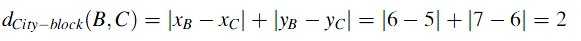
\includegraphics[scale=0.6]{images/Manhattan.jpg}\\
		\end{center}
	\end{figure}
	
	
	
	

	
\end{itemize}


\subsection{Other Measures}
\begin{itemize}
\item When working with metric (or ordinal) data, researchers frequently use
the \textbf{\textit{Chebychev distance}}, which is the maximum of the absolute difference in the
clustering variables� values. This distance measure may be appropriate in cases when we want to define two objects as "different" if they are different on any one of the dimensions. The Chebychev distance is computed as:
\[\mbox{distance(x,y)} = \mbox{Maximum}|x_i - y_i|\] For B and C, this result is:

\begin{figure}[h!]
	\begin{center}
		% Requires \usepackage{graphicx}
		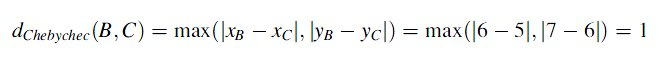
\includegraphics[scale=0.6]{images/Chebyshev.jpg}\\
	\end{center}
\end{figure}


\item \textbf{Power distance.} Sometimes we may want to increase or decrease the progressive weight that is placed on dimensions on which the respective objects are very different. This can be accomplished via the power distance. The power distance is computed as:
\[\mbox{distance(x,y)}  = (\sum_i |x_i - y_i|^p)^{1/r}\]

Parameter p controls the progressive weight that is placed on differences on individual dimensions, parameter r controls the progressive weight that is placed on larger differences between objects. If r and p are equal to 2, then this distance is equal to the Euclidean distance.

A few example calculations may demonstrate how this measure "behaves." 
\begin{itemize}
\item[$\ast$] Parameter p controls the progressive weight that is placed on differences on individual dimensions
\item[$\ast$] parameter r controls the progressive weight that is placed on larger differences between objects
\item[$\ast$] If r and p are equal to 2, then this distance is equal to the Euclidean distance.
\end{itemize}

\item \textbf{Percent disagreement.} This measure is particularly useful if the data for the dimensions included in the analysis are categorical in nature. This distance is computed as:
distance(x,y) = (Number of xi  yi)/ i
	\item There are other distance measures such as the Angular, Canberra or Mahalanobis
	distance. In many situations, the \textbf{\textit{Mahalanobis
			distance}} is desirable as this measure compensates for \textbf{\textit{multi-collinearity}}
	between the clustering variables. However, it is unfortunately not menu-accessible
	in SPSS.
\end{itemize}
%-------------------------------------------------------------------------------------------------%
\section{Standardizing the Variables}
% % Moved to CA Notes
Note that Euclidean (and squared Euclidean) distances are usually computed from raw data, and not from standardized data. This method has certain advantages (e.g., the distance between any two objects is not affected by the addition of new objects to the analysis, which may be outliers). However, the distances can be greatly affected by differences in scale among the dimensions from which the distances are computed. 

For example, if one of the dimensions denotes a measured length in centimeters, and you then convert it to millimeters (by multiplying the values by 10), the resulting Euclidean or squared Euclidean distances (computed from multiple dimensions) can be greatly affected (i.e., biased by those dimensions which have a larger scale), and consequently, the results of cluster analyses may be very different. Generally, it is good practice to transform the dimensions so they have similar scales.

\begin{itemize}
	\item If variables are measured on different scales, variables with large values contribute
	more to the distance measure than variables with small values. 
	\item In this example, both
	variables are measured on the same scale, so that�s not much of a problem, assuming
	the judges use the scales similarly. But if you were looking at the distance between two
	people based on their IQs and incomes in dollars, you would probably find that the
	differences in incomes would dominate any distance measures. \item (A difference of only
	\$100 when squared becomes 10,000, while a difference of 30 IQ points would be only
	900. I�d go for the IQ points over the dollars!).
	
	\item Variables that are measured in large numbers will contribute to the distance more than variables recorded in smaller
	numbers.
	
	\item In the hierarchical clustering procedure in SPSS, you can standardize variables in
	different ways. You can compute standardized scores or divide by just the standard
	deviation, range, mean, or maximum. This results in all variables contributing more
	equally to the distance measurement. That�s not necessarily always the best strategy,
	since variability of a measure can provide useful information. 
	
\end{itemize}
%----------------------------------------------------- %
\newpage
\section{Standardized Distance}

Let us consider measuring the distances between between two points using
the three continuous variables pollution, depth and temperature. Let us suppose that a difference of 4.1 in terms of pollution is considered quite large and unusual, while a difference of 48 in terms of depth is large, but not particularly unusual.
What would happen if we applied the Euclidean distance formula to measure distance between two cases.
\begin{center}
	\begin{tabular}{|c|c|c|}
		\hline
		% after \\: \hline or \cline{col1-col2} \cline{col3-col4} ...
		Variables & case 1 & case 2 \\ \hline 
		Pollution & 6.0 & 1.9 \\
		Depth & 51 & 99 \\
		Temp & 3.0 & 2.9 \\
		\hline
	\end{tabular}
\end{center}

Here is the calculation for Euclidean Distance:
\[ d = \sqrt{(6.0 - 1.9)^2 + (51 - 99)^2 + (3.0 - 2.9)^2}   \]
\[ d = \sqrt{16.81 + 2304 + 0.01} = \sqrt{2320.82} = 48.17 \]
\noindent The contribution of the second variable depth to this calculation is huge ,therefore one could say
that the distance is practically just the absolute difference in the depth values (equal to
$|51-99|$ = 48) with only tiny additional contributions from pollution and temperature. These three variables are on
completely different scales of measurement and the larger depth values have larger differences, so they will dominate in the calculation of Euclidean distances.


\noindent The approach to take here is \textbf{standardization}, which is is necessary to balance out the contributions, and the
conventional way to do this is to transform the variables so they all have the same variance
of 1. At the same time we \textbf{\textit{center}} the variables at their means, this centering is not
necessary for calculating distance, but it makes the variables all have mean zero and thus
easier to compare. 

\noindent The transformation commonly called standardization is thus as follows:

\[\mbox{standardized value} = \frac{\mbox{observed value - mean}}{ \mbox{standard deviation}}\]
\begin{center}
	\begin{tabular}{|c|c|c|c|c|c|c|}
		\hline
		% after \\: \hline or \cline{col1-col2} \cline{col3-col4} ...
		Variables & Case 1 & Case 2 & Mean & Std. Dev & Case 1 (std) & Case 2 (std) \\ \hline
		Pollution & 6.0 & 1.9 & 4.517	&	2.141	&	0.693	&	-1.222	\\
		Depth & 51 & 99 & 74.433	&	15.615	&	-1.501	&	1.573	\\
		Temp & 3.0 & 2.9 & 3.057	&	0.281	&	-0.201	&	-0.557	\\
		\hline
	\end{tabular}
\end{center}

\[ d_{std} =  \sqrt{(0.693 - (- 1.222))^2 + (-1.501-1.573)^2 + (-0.201-(-0.557))^2} \]

\[ d_{std} = \sqrt{3.667 + 9.449 + 0.127} = \sqrt{13.243} = 3.639 \]

Pollution and temperature have higher contributions than before but depth still plays the
largest role in this particular example, even after standardization. But this contribution is
justified now, since it does show the biggest standardized difference between the samples. 
\subsection{Logarithmic Transformation}
As as alternative to scaling or standardization, the user may opt to use the logarithm of a value, rather than the value itself.
%--------------------------------------------------------------------------------------%


\section{Standardizing the Variables}
If variables are measured on different scales, variables with large values contribute
more to the distance measure than variables with small values. In this example, both
variables are measured on the same scale, so that�s not much of a problem, assuming
the judges use the scales similarly. 

But if you were looking at the distance between two people based on their IQs and incomes in dollars, you would probably find that the
differences in incomes would dominate any distance measures. (A difference of only
\$100 when squared becomes 10,000, while a difference of 30 IQ points would be only
900. I�d go for the IQ points over the dollars!).

Variables that are measured in large numbers will contribute to the distance more than variables recorded in smaller
numbers.
%-------------------------------------------------------------------------------------------------%
In the hierarchical clustering procedure in SPSS, you can standardize variables in
different ways. You can compute standardized scores or divide by just the standard
deviation, range, mean, or maximum. This results in all variables contributing more
equally to the distance measurement. That�s not necessarily always the best strategy,
since variability of a measure can provide useful information. 
%-------------------------------------------------------------------------------------------------%

\newpage

\section{Cluster Analysis : Proximity Matrices}

Using \textbf{\textit{nearest neighbour}} linkage, describe how the agglomeration schedule based on the following 
proximity matrix. With nearest neighbour, a case is assigned to the cluster of the case with which it has the shortest distance. Cluster are also joined on this basis.


% latex table generated in R 2.15.2 by xtable 1.7-1 package
% Tue May 14 19:17:33 2013
\begin{table}[ht]
	\centering
	\begin{tabular}{|r|rrrrrrrrrr|}
		\hline
		Case & 1 & 2 & 3 & 4 & 5 & 6 & 7 & 8 & 9 & 10 \\
		\hline
		1 & 0.00 & \textbf{4.82} & 89.39 & 85.97 & 46.26 & 71.87 & 56.42 & 23.75 & 31.57 & 11.70 \\
		2 & \textbf{4.82} & 0.00 & 94.24 & 38.96 & \textbf{5.55} & 35.07 & 74.52 & 71.27 & 61.84 & \textbf{4.84} \\
		3 & 89.39 & 94.24 & 0.00 & 57.65 & 27.27 & 25.31 & 20.89 & \textbf{2.84} & 63.50 & 89.39 \\
		4 & 85.97 & 38.96 & 57.65 & 0.00 & \textbf{22.94} & \textbf{7.13} & 70.49 & 23.09 & \textbf{12.75} & 85.97 \\
		5 & 46.26 & \textbf{5.55} & 27.27 & \textbf{22.94} & 0.00 & 39.44 & 17.43 & 79.22 & 14.47 & 46.26 \\
		6 & 71.87 & 35.07 & 25.31 & \textbf{7.13} & 39.44 & 0.00 & 27.50 & 30.65 & 13.34 & 71.87 \\
		7 & 56.42 & 74.52 & 20.89 & 70.49 & 17.43 & 27.50 & 0.00 & 91.16 & 44.92 & \textbf{6.42} \\
		8 & 23.75 & 71.27 & \textbf{2.84} & 23.09 & 79.22 & 30.65 & 91.16 & 0.00 & \textbf{3.18} & 23.75 \\
		9 & 31.57 & 61.84 & 63.50 & \textbf{12.75} & 14.47 & 13.34 & 44.92 & \textbf{3.18} & 0.00 & 31.57 \\
		10 & 11.70 & \textbf{4.84} & 89.39 & 85.97 & 46.26 & 71.87 & \textbf{6.42} & 23.75 & 31.57 & 0.00 \\
		\hline
	\end{tabular}
\end{table}


\begin{itemize}
	\item The closest pair in terms of distance (2.84) are cases 3 and 8. So this is the first linkage.
	\item The next closest pair (3.18) are 8 and 9. The next linkage joins case 9 to 3 and 8.
	\item The next closest pair (4.82) are 1 and 2. So this is the next linkage. [ So far (3,8,9) and (2,10) ] 
	\item The next closest pair (4.84) are 2 and 10. The next linkage joins case 1 to 2 and 10.
	\item The next closest pair (5.55) are 2 and 5. The next linkage joins case 5 to 1, 2 and 10. [ So far (3,8,9) and (1,2,5,10)]
	\item The next closest pair (6.42) are 7 and 10. The next linkage joins case 7 to 1, 2, 5 and 10.
	\item The next closest pair (7.13) are 4 and 6. The next linkage joins case 4 to 6. [ So far (3,8,9), (4,6) and (1,2,5,10) All cases are in clusters. This is a 3 cluster solution. ]
	\item The next closest pair (11.70) are 1 and 10. Disregard, because they are already clustered together.
	\item The next closest pair (19.44) are 4 and 9. This joins cluster (4,6) to cluster (3,8,9) [ So far (3,4,6,8,9) and (1,2,5,10). This is a 2 cluster solution.]
	\item The next closest pairing is 4 and 5. This linkage joins all cases together in one cluster.
\end{itemize}

\newpage
\section{Linkage Methods for Cluster Analysis}
Having selected how we will measure distance, we must now choose the clustering algorithm, i.e. the rules that govern between which points distances are measured to determine cluster membership. There are many methods available, the criteria used differ and hence
different classifications may be obtained for the same data. This is important since it tells us that, although cluster analysis may provide an objective method for the clustering of cases, there can be subjectivity in the choice of method. 

The linkage distances are calculated by SPSS. The goal of the clustering algorithm is to join objects together into successively larger clusters, using some measure of similarity or distance. SPSS provides seven clustering algorithms, the most commonly used one being  \textbf{\textit{Ward's method}}.


\subsection{Nearest neighbour method} 
\begin{itemize}
	\item A commonly used approach in hierarchical clustering is \textbf{\textit{Ward�s linkage method}}.
	This approach does not combine the two most similar objects successively. Instead,
	those objects whose merger increases the overall within-cluster variance to the
	smallest possible degree, are combined. If you expect somewhat equally sized
	clusters and the data set does not include outliers, you should always use Ward�s
	method.
	
	We will use the Ward's linkage method for laboratory exercises.
	
	\item Other most popular
	agglomerative clustering procedures include the following:
	\begin{description}
		\item[Single linkage (nearest neighbor)]: The distance between two clusters corresponds
		to the shortest distance between any two members in the two clusters.
		\begin{figure}[h!]
			\begin{center}
				% Requires \usepackage{graphicx}
				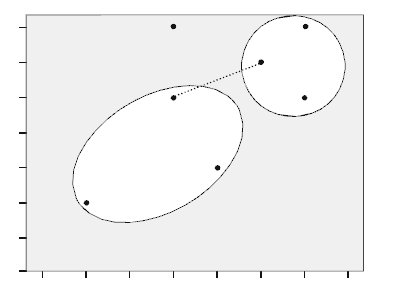
\includegraphics[scale=0.4]{images/Link1.jpg}\\
			\end{center}
		\end{figure}
		\item[Complete linkage (furthest neighbor)]: The oppositional approach to single
		linkage assumes that the distance between two clusters is based on the longest
		distance between any two members in the two clusters.
		\begin{figure}[h!]
			\begin{center}
				% Requires \usepackage{graphicx}
				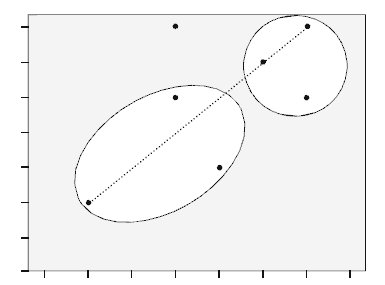
\includegraphics[scale=0.4]{images/Link2.jpg}\\
			\end{center}
		\end{figure}
		\item[Average linkage] : The distance between two clusters is defined as the average
		distance between all pairs of the two clusters� members.
		\begin{figure}[h!]
			\begin{center}
				% Requires \usepackage{graphicx}
				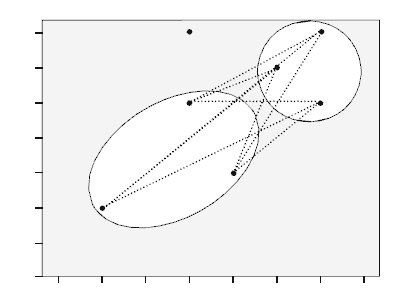
\includegraphics[scale=0.4]{images/Link3.jpg}\\
			\end{center}
		\end{figure}
		\newpage
		\item[Centroid] : In this approach, the geometric center (centroid) of each cluster is
		computed first. The distance between the two clusters equals the distance between
		the two centroids.
		\begin{figure}[h!]
			\begin{center}
				% Requires \usepackage{graphicx}
				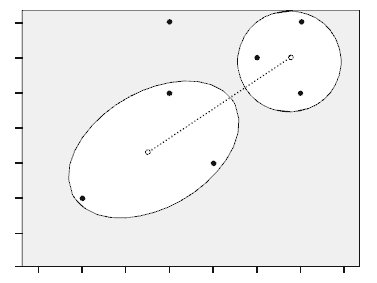
\includegraphics[scale=0.4]{images/Link4.jpg}\\
			\end{center}
		\end{figure}
	\end{description}
	Each of these linkage algorithms can yield totally different results when used on the same data set, as each has its specific properties. As the single linkage algorithm is based on minimum distances, it tends to form one large cluster with the other clusters containing only one or few objects each. We can make use of this \textbf{\textit{chaining effect}} to detect outliers, as these will be merged with the remaining objects � usually at very large distances � in the last steps of the analysis. Generally, single linkage is considered the most versatile algorithm.
	
	Conversely, the complete linkage method is strongly affected by outliers, as it is based on maximum distances. Clusters produced by this method are likely to be rather compact and tightly clustered. The average linkage and centroid algorithms tend to produce clusters with rather low within-cluster variance and similar sizes.
	However, both procedures are affected by outliers, though not as much as complete linkage.
\end{itemize}
\textit{(Also known as the single linkage method)}.\\
In this method the distance between two clusters is defined to be the distance between
the two closest members, or neighbours. This method is relatively simple but is often
criticised because it doesn�t take account of cluster structure and can result in a problem
called chaining whereby clusters end up being long and straggly. However, it is better
than the other methods when the natural clusters are not spherical or elliptical in shape.

\subsection{Nearest neighbour method} 
(Also known as the single linkage method).\\
In this method the distance between two clusters is defined to be the distance between
the two closest members, or neighbours. This method is relatively simple but is often
criticised because it doesn�t take account of cluster structure and can result in a problem
called chaining whereby clusters end up being long and straggly. However, it is better
than the other methods when the natural clusters are not spherical or elliptical in shape.

\subsection{Furthest neighbour method}
\textit{(Also known as the complete linkage method)}.\\
In this case the distance between two clusters is defined to be the maximum distance
between members  i.e. the distance between the two subjects that are furthest apart.
This method tends to produce compact clusters of similar size but, as for the nearest
neighbour method, does not take account of cluster structure. It is also quite sensitive
to outliers.


\subsection{Average (between groups) linkage method }
\textit{(sometimes referred to as Unweighted Pair Group Method with Arithmetic Mean (UPGMA)).}\\
The distance between two clusters is calculated as the average distance between all pairs
of subjects in the two clusters. This is considered to be a fairly robust method.

\subsection{Centroid method}
Here the centroid (mean value for each variable) of each cluster is calculated and the
distance between centroids is used. Clusters whose centroids are closest together are
merged. This method is also fairly robust.

\subsection{Centroid method}
Here the centroid (mean value for each variable) of each cluster is calculated and the
distance between centroids is used. Clusters whose centroids are closest together are
merged. This method is also fairly robust.

\subsection{Ward�s method}
In this method all possible pairs of clusters are combined and the sum of the squared
distances within each cluster is calculated. This is then summed over all clusters. The
combination that gives the lowest sum of squares is chosen. This method tends to
produce clusters of approximately equal size, which is not always desirable. It is also
quite sensitive to outliers. Despite this, it is one of the most popular methods, along
with the average linkage method.

%\subsection{Ward's Method}
%This method is distinct from other methods because it uses an \textbf{\textit{analysis of variance}} approach to evaluate the distances between clusters. In general, this method is very efficient.
%
%Cluster membership is assessed by calculating the total sum of squared deviations from the mean of a cluster. The criterion for fusion is that it should produce the smallest possible increase
%in the error sum of squares.
%
%
%
%\subsection{Ward's Linkage}
%
%Ward's linkage is a method for hierarchical cluster analysis . The idea has much in common with analysis of variance (ANOVA). The linkage function specifying the distance between two clusters is computed as the increase in the "error sum of squares" (ESS) after fusing two clusters into a single cluster. Ward's Method seeks to choose the successive clustering steps so as to minimize the increase in ESS at each step.


\subsection{Ward�s Linkage method (IMPORTANT)}
In this method all possible pairs of clusters are combined and the sum of the squared
distances within each cluster is calculated. This is then summed over all clusters. The
combination that gives the lowest sum of squares is chosen. This method tends to
produce clusters of approximately equal size, which is not always desirable. It is also
quite sensitive to outliers. Despite this, it is one of the most popular methods, along
with the average linkage method.

%\subsection{Ward's Method}
%This method is distinct from other methods because it uses an \textbf{\textit{analysis of variance}} approach to evaluate the distances between clusters. In general, this method is very efficient.
%
%Cluster membership is assessed by calculating the total sum of squared deviations from the mean of a cluster. The criterion for fusion is that it should produce the smallest possible increase
%in the error sum of squares.
%
%
%
%\subsection{Ward's Linkage}
%
%Ward's linkage is a method for hierarchical cluster analysis . The idea has much in common with analysis of variance (ANOVA). The linkage function specifying the distance between two clusters is computed as the increase in the "error sum of squares" (ESS) after fusing two clusters into a single cluster. Ward's Method seeks to choose the successive clustering steps so as to minimize the increase in ESS at each step.


%
%\subsection{Applications of Cluster Analysis}
%
%In medicine, the clustering of symptoms and diseases leads to taxonomies of illnesses. In the field of business, clusters of consumer segments are often sought for successful marketing strategies. Biologists have to organize the different species of animals before a meaningful description of the differences between animals is possible.

%\subsection{Cluster Analysis as a Statistical Tool}




\subsection{Summary of Linkage methods}
\begin{itemize}
	\item  Single linkage (minimum distance)
	\item  Complete linkage (maximum distance)
	\item  Average linkage
\end{itemize}

%http://www.rdg.ac.uk/~aes02mm/supermarket.sav

\subsubsection{Ward's method}
\begin{itemize}
	\item  Compute sum of squared distances within clusters
	\item  Aggregate clusters with the minimum increase in the
	overall sum of squares
\end{itemize}
\subsubsection{Centroid method}
The distance between two clusters is defined as the
difference between the centroids (cluster averages)


% http://www.norusis.com/pdf/SPC_v13.pdf
 \section{Clustering Algorithm}
 To better understand how a clustering algorithm works, let�s manually examine
 some of the single linkage procedure�s calculation steps. We start off by looking at
 the initial (Euclidean) distance matrix displayed previously.
 
 \begin{figure}[h!]
 	\begin{center}
 		% Requires \usepackage{graphicx}
 		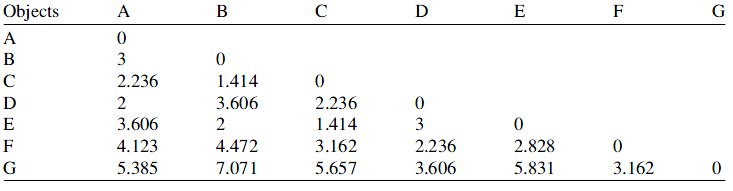
\includegraphics[scale=0.6]{images/DistanceMatrix.jpg}\\
 	\end{center}
 \end{figure}
 
 \begin{itemize}
 	\item In the very first step, the two
 	objects exhibiting the smallest distance in the matrix are merged. Note that we
 	always merge those objects with the smallest distance, regardless of the clustering
 	procedure (e.g., single or complete linkage). (N.B. In the following example, ties will be broken at random.)
 	\item As we can see, this happens to two
 	pairs of objects, namely B and C (\textbf{d(B, C)} = 1.414), as well as C and E (\textbf{d(C, E)} =
 	1.414). In the next step, we will see that it does not make any difference whether we
 	first merge the one or the other, so let�s proceed by forming a new cluster, using
 	objects B and C.
 	\begin{figure}[h!]
 		\begin{center}
 			% Requires \usepackage{graphicx}
 			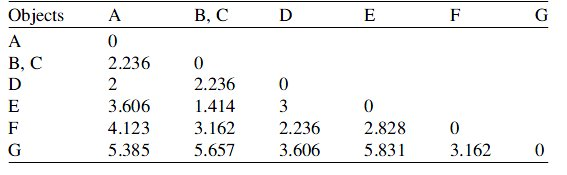
\includegraphics[scale=0.6]{images/DistanceMatrix2.jpg}\\
 		\end{center}
 	\end{figure}
 	\item Having made this decision, we then form a new distance matrix by considering
 	the single linkage decision rule as discussed above. According to this rule, the
 	distance from, for example, object A to the newly formed cluster is the minimum of
 	\textbf{d(A, B)} and \textbf{d(A, C)}. As \textbf{d(A, C)} is smaller than d(A, B), the distance from A to the
 	newly formed cluster is equal to d(A, C); that is, 2.236.
 	\item We also compute the
 	distances from cluster [B,C] (clusters are indicated by means of squared brackets)
 	to all other objects (i.e. D, E, F, G) and simply copy the remaining distances � such
 	as \textbf{d(E, F)} � that the previous clustering has not affected.
 	\begin{figure}[h!]
 		\begin{center}
 			% Requires \usepackage{graphicx}
 			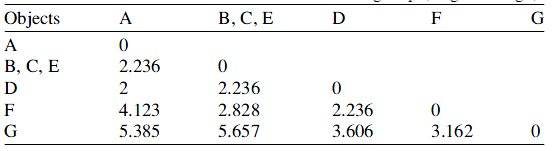
\includegraphics[scale=0.6]{images/DistanceMatrix3.jpg}\\
 		\end{center}
 	\end{figure}
 	\item Continuing the clustering procedure, we simply repeat the last step by merging
 	the objects in the new distance matrix that exhibit the smallest distance (in this case,
 	the newly formed cluster [B, C] and object E) and calculate the distance from this
 	cluster to all other objects.
 	\begin{figure}[h!]
 		\begin{center}
 			% Requires \usepackage{graphicx}
 			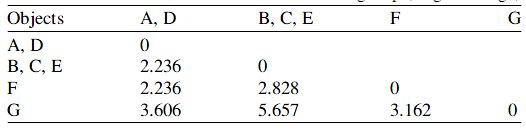
\includegraphics[scale=0.6]{images/DistanceMatrix4.jpg}\\
 		\end{center}
 	\end{figure}
 	\item We continue in the same fashion until one cluster is left. By following the single linkage procedure, the last steps involve the merger
 	of cluster [A,B,C,D,E,F] and object G at a distance of 3.162.
 	\begin{figure}[h!]
 		\begin{center}
 			% Requires \usepackage{graphicx}
 			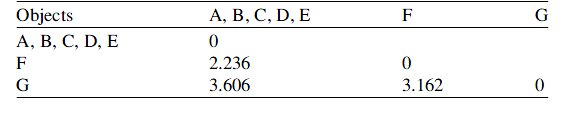
\includegraphics[scale=0.6]{images/DistanceMatrix5.jpg}\\
 		\end{center}
 	\end{figure}
 	\begin{figure}[h!]
 		\begin{center}
 			% Requires \usepackage{graphicx}
 			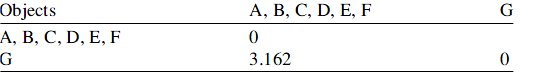
\includegraphics[scale=0.6]{images/DistanceMatrix6.jpg}\\
 		\end{center}
 	\end{figure}
 \end{itemize}
 \newpage
 
 
 

\section{Dendrograms}

The dendrogram is a tree-structured graphical representation, used to visualize of the results of \textbf{\textit{hierarchical cluster analysis}} . This is a tree-like plot where each step of hierarchical clustering is represented as a joining (or fusion) of two branches of the tree into a single one. The branches represent clusters obtained on each step of hierarchical clustering. The result of a clustering is presented either as the \textbf{\textit{distance}} or the similarity between the clustered rows or columns depending on the selected distance measure.


%----------------------------------------------------------%
% http://www2.statistics.com/resources/glossary/h/hclusteran.php

% http://mlsc.lboro.ac.uk/resources/statistics/Clusteranalysis.pdf


\section{SPSS Implementation and Output}

Hierarchical Cluster Analysis is implemented by the \textbf{classify} option on the \textbf{analyse} menu.
Three options shall appear. Select Hierarchical.

We performed a hierarchical cluster analysis in SPSS, selecting all the variables (except categorical variables) in the \textbf{Variable(s)} box. We can label the cases by a categorical variable. 

We shall further requested the Dendrogram in the output. We changed all
variables to z-scores to yield equal metrics and equal weighting, selected the Squared Euclidean distance
(the default) method of determining distance between clusters and the \textbf{Ward's method} for
clustering, and saved a 3-cluster solution as a new variable.

\subsection{Proximity matrix}
The output will print distances or similarities computed for any pair of cases. We will not be covering this in detail.

\subsection{Cluster Membership}
This box allows you to specify a set number of clusters. If you have a
hypothesis about how many clusters there are, you can specify a set number of clusters, or
create a number of clusters within a range.

\subsection{Icicle Plot} Default choice by SPSS. Icicle plots visually represent information on the agglomeration
schedule. You can select that all clusters are included in the icicle plot, or restrict it to a range of
clusters. Also, you can read the plot from bottom up (vertical orientation) or from left to right
(horizontal orientation).

\subsection{Measure} There are different distance measure choices depending on the level of measurement
of the data: interval, count, or binary.

For nearly all of this module example,the data were on an interval scale, and the squared euclidean measure will suffice.


\newpage
\subsection{SPSS Agglomeration Schedule}
The procedure followed by cluster analysis at Stage 1 is to cluster the two cases that have the smallest
squared Euclidean distance between them. Then SPSS will recompute the distance measures between all
single cases and clusters (there is only one cluster of two cases after the first step). Next, the 2 cases (or
clusters) with the smallest distance will be combined, yielding either 2 clusters of 2 cases (with 17 cases
unclustered) or one cluster of 3 (with 18 cases unclustered).  This process continues until all cases are clustered into a single group.
\begin{center}
\begin{figure}[h!]
	% Requires \usepackage{graphicx}
	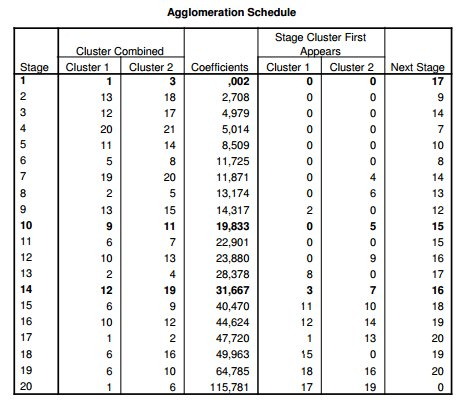
\includegraphics[scale=0.7]{images/AggloSc}\\
	\caption{SPSS Agglomeration Schedule}
\end{figure}
\end{center}



For the sake of clarify, we will explain Stages 1, 10, and 14.


\subsubsection*{Stage 1}
\begin{itemize}
\item At Stage 1, Case 1 is clustered with Case 3. The squared Euclidean distance between these two cases is
.002. \item Neither variable has been previously clustered (the two zeros under Cluster 1 and Cluster 2), and the
next stage (when the cluster containing Case 1 combines with another case) is Stage 17. 
\item (Note that at Stage
17, Case 2 joins the Case-1 cluster.)
\end{itemize}


\subsubsection*{Stage 10}
\begin{itemize}
\item At Stage 10, Case 9 joins the Case-11 cluster (Case 11 was previously clustered with Case 14 back in Stage
5, thus creating a cluster of 3 cases: Cases 9, 11, and 14). \item The squared Euclidean distance between Case 9
and Case-11 cluster is 19.833. Case 9 has not been previously clustered (the zero under Cluster 1), and
Case 11 was previously clustered at Stage 5. \item The next stage (when the cluster containing Case 9 clusters) is
Stage 15 (when it combines with the Case-6 cluster).
\end{itemize}


\subsubsection*{Stage 14}
\begin{itemize}
\item At Stage 14, the clusters containing Cases 12 and 19 are joined, Case 12 has been previously clustered with
Case 17, and Case 19 had been previously clustered with Cases 20 and 21, thus forming a cluster of 5 cases
(Cases 12, 17, 19, 20, 21). 
\item The squared Euclidean distance between the two joined clusters is 31.667. Case
12 was previously joined at Stage 3 with Case 17. Case 19 was previously joined at Stage 7 with the Case-
20 cluster. 
\item The next stage when the Case-12 cluster will combine with another case/cluster is Stage 16
(when it joins with the Case-10 cluster).
\end{itemize}


\begin{figure}
  % Requires \usepackage{graphicx}
  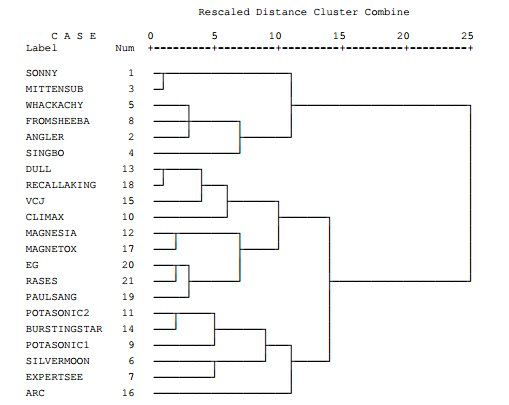
\includegraphics[scale=0.7]{images/Dendro}\\
  \caption{Corresponding Dendrogram}
\end{figure}

The branching-type nature of the Dendrogram allows you to trace backward or forward to any individual
case or cluster at any level. It, in addition, gives an idea of how great the distance was between cases or
groups that are clustered in a particular step, using a 0 to 25 scale along the top of the chart. While it is
difficult to interpret distance in the early clustering phases (the extreme left of the graph), as you move to
the right relative distance become more apparent. The bigger the distances before two clusters are joined,
the bigger the differences in these clusters. To find a membership of a particular cluster simply trace
backwards down the branches to the name.

\newpage


\newpage
\section{Non-Hierarchical Clustering}
This method of clustering is very different from the hierarchical clustering and Ward method, which are applied when there is no prior knowledge of how many clusters there may be or what they are characterized by. The k-means clustering approach is used when you already have hypotheses concerning the number of clusters in your cases or variables. For example, you may want to specify exactly three clusters that are to be as distinct as possible.

This is the type of research question that can be addressed by the k-means clustering algorithm. In general, the k-means method will produce the exact k different clusters demanded of greatest possible distinction. Very often, both the hierarchical and the k-means techniques are used successively.
\begin{itemize}
	\item Ward's method is used to get some sense of the possible number of clusters and the way they merge as seen from the dendrogram.
	\item Then the clustering is rerun with only a chosen optimum number in which to place all
	the cases (i.e. k means clustering).
\end{itemize}
%-------------------------------------------------------------------------------------------------%
In these methods the desired number of clusters is specified in advance and the `best' solution
is chosen. The steps in such a method are as follows:
\begin{itemize}
	\item[1] Choose initial cluster centres (essentially this is a set of observations that are far apart
	� each subject forms a cluster of one and its centre is the value of the variables for
	that subject).
	\item[2] Assign each subject to its `nearest' cluster, defined in terms of the distance to the
	centroid.
	\item[3] Find the centroids of the clusters that have been formed
	\item[4] Re-calculate the distance from each subject to each centroid and move observations that
	are not in the cluster that they are closest to.
	\item[5] Continue until the centroids remain relatively stable.
\end{itemize}
%-------------------------------------------------------------------------------------------------%
Non-hierarchical cluster analysis tends to be used when large data sets are involved. It is
sometimes preferred because it allows subjects to move from one cluster to another (this is
not possible in hierarchical cluster analysis where a subject, once assigned, cannot move to a
different cluster). Two disadvantages of non-hierarchical cluster analysis are: 
\begin{itemize}
	\item[1]it is often
	diffcult to know how many clusters you are likely to have and therefore the analysis may have
	to be repeated several times 
	\item[2] it can be very sensitive to the choice of initial cluster centres. Again, it may be worth trying di?erent ones to see what impact this has.
\end{itemize}
%-------------------------------------------------------------------------------------------------%

\section{Non-Hierarchical Clustering (Kmeans)}
This method of clustering is very different from the hierarchical clustering and Ward method, which are applied when there is no prior knowledge of how many clusters there may be or what they are characterized by. The k-means clustering approach is used when you already have hypotheses concerning the number of clusters in your cases or variables. For example, you may want to specify exactly three clusters that are to be as distinct as possible.

This is the type of research question that can be addressed by the k-means clustering algorithm. In general, the k-means method will produce the exact k different clusters demanded of greatest possible distinction. Very often, both the hierarchical and the k-means techniques are used successively.
\begin{itemize}
\item Ward's method is used to get some sense of the possible number of clusters and the way they merge as seen from the dendrogram.
\item Then the clustering is rerun with only a chosen optimum number in which to place all
the cases (i.e. k means clustering).
\end{itemize}

In these methods the desired number of clusters is specified in advance and the `best' solution
is chosen. The steps in such a method are as follows:
\begin{itemize}
\item[1] Choose initial cluster centres (essentially this is a set of observations that are far apart
� each subject forms a cluster of one and its centre is the value of the variables for
that subject).
\item[2] Assign each subject to its `nearest' cluster, defined in terms of the distance to the
centroid.
\item[3] Find the centroids of the clusters that have been formed
\item[4] Re-calculate the distance from each subject to each centroid and move observations that
are not in the cluster that they are closest to.
\item[5] Continue until the centroids remain relatively stable.
\end{itemize}

Non-hierarchical cluster analysis tends to be used when large data sets are involved. It is
sometimes preferred because it allows subjects to move from one cluster to another (this is
not possible in hierarchical cluster analysis where a subject, once assigned, cannot move to a
different cluster). Two disadvantages of non-hierarchical cluster analysis are: 
\begin{itemize}
\item[1]it is often
diffcult to know how many clusters you are likely to have and therefore the analysis may have
to be repeated several times 
\item[2] it can be very sensitive to the choice of initial cluster centres. Again, it may be worth trying di?erent ones to see what impact this has.
\end{itemize}


 \section{K-Means Clustering}
 \begin{itemize}
 	\item Hierarchical clustering requires a distance or similarity matrix between all pairs of cases. That's an extremely large matrix if you have tens of thousands of cases in your data file.
 	
 	\item A clustering method that doesn't require computation of all possible distances is k-means clustering. It differs from hierarchical clustering in several ways. You have to know in advance the number of clusters you want. You can't get solutions for a range of cluster numbers unless you rerun the analysis for each different number of clusters.
 	
 	\item The algorithm repeatedly reassigns cases to clusters, so the same case can move from cluster to cluster during the analysis. In agglomerative hierarchical clustering, on the other hand, cases are added only to existing clusters. They are forever captive in their cluster, with a widening circle of ``neighbours".
 	
 	\item The algorithm is called \textbf{k-means}, where \textbf{k} is the number of clusters you want, since a case is assigned to the cluster for which its distance to the cluster mean is the smallest.
 	
 	\item The k-means algorithm follows an entirely different concept than the hierarchical methods
 	discussed before. This algorithm is not based on distance measures such as
 	Euclidean distance or city-block distance, but uses the \textbf{\textit{within-cluster variation}} as a measure to form homogenous clusters. Specifically, the procedure aims at segmenting
 	the data in such away that the within-cluster variation isminimized.Consequently,we
 	do not need to decide on a distance measure in the first step of the analysis.
 	
 	\item The action in the algorithm centers around finding the k-means. You start out with an initial set of means and classify cases based on their distances to the centers.
 	
 	\item Next, you compute the cluster means again, using the cases that are assigned to the cluster; then, you reclassify all cases based on the new set of means. You keep repeating this step until cluster means don't change much between successive steps.
 	
 	\item Finally, you calculate the means of the clusters once again and assign the cases to their permanent clusters.
 \end{itemize}
 %------------------------------------------------------------------%
 \subsection{Initial Cluster Centres}
 The first step in k-means clustering is finding the k centres. This is done iteratively. You start with an initial set of centres and then modify them until the change between two iterations is small enough.
 
 If you have good guesses for the centres, you can use those
 as initial starting points; otherwise, you can let SPSS find k cases that are well separated and use these values as initial cluster centers. (i.e. The clustering process starts by randomly assigning objects to a number of
 clusters).
 
 
 
 K-means clustering is very sensitive to outliers, since they will usually be selected as initial cluster centers. This will result in outliers forming clusters with small numbers of cases. Before you start a cluster analysis, screen the data for outliers and remove them from the initial analysis. The solution may also depend on the order of the cases in the data.
 
 After the initial cluster centers have been selected, each case is assigned to the closest
 cluster, based on its distance from the cluster centers. After all of the cases have been
 assigned to clusters, the cluster centers are recomputed, based on all of the cases in the
 cluster.
 
 The cases are then successively reassigned to other clusters to minimize the within-cluster variation, which is basically the (squared) distance from each observation to the center of the associated cluster. If the reallocation of an case to another cluster decreases the within-cluster variation, this case is reassigned
 to that cluster.
 
 Case assignment is done again, using these updated cluster centers. You keep
 assigning cases and recomputing the cluster centers until no cluster center changes
 appreciably or the maximum number of iterations (10 by default) is reached.
 \newpage
 \subsection{Demonstration of k-means}
 In this example, two cluster centers are randomly
 initiated, which CC1 (first cluster) and CC2 (second cluster).
 \begin{figure}[h!]
 	\begin{center}
 		% Requires \usepackage{graphicx}
 		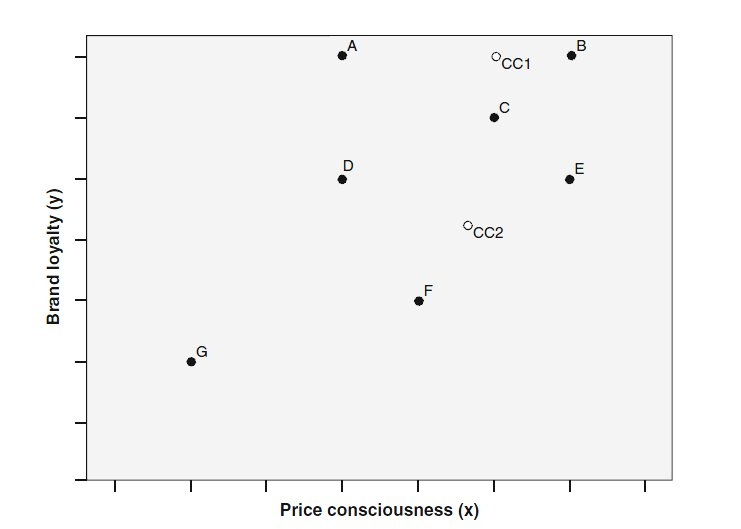
\includegraphics[scale=0.4]{images/kmeans1.jpg}\\
 	\end{center}
 \end{figure}
 \begin{figure}[h!]
 	\begin{center}
 		% Requires \usepackage{graphicx}
 		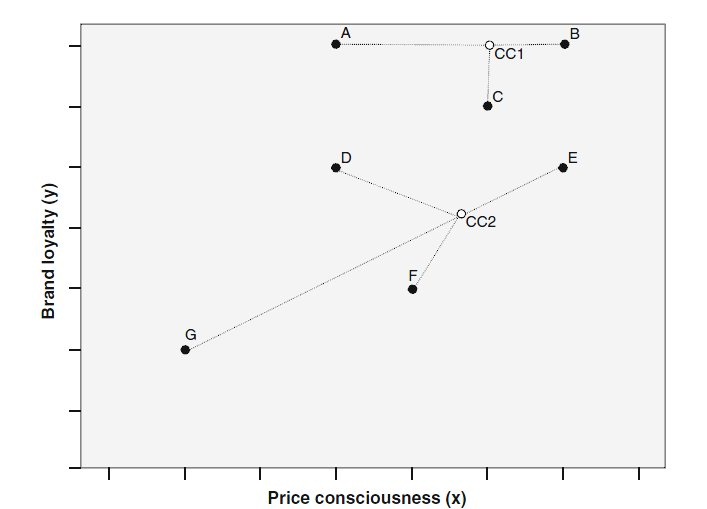
\includegraphics[scale=0.4]{images/kmeans2.jpg}\\
 	\end{center}
 \end{figure}
 Euclidean distances are computed from the cluster
 centers to every single object. Each object is then assigned to the cluster center with
 the shortest distance to it.
 
 In this example, objects A, B, and C are
 assigned to the first cluster, whereas objects D, E, F, and G are assigned to the
 second. We now have our initial partitioning of the objects into two clusters.
 Based on this initial partition, each cluster�s geometric center (i.e., its centroid)
 is computed (third step). This is done by computing the mean values of the objects
 contained in the cluster (e.g., A, B, C in the first cluster) regarding each of the variables
 (in this example: price consciousness and brand loyalty).
 \begin{figure}[h!]
 	\begin{center}
 		% Requires \usepackage{graphicx}
 		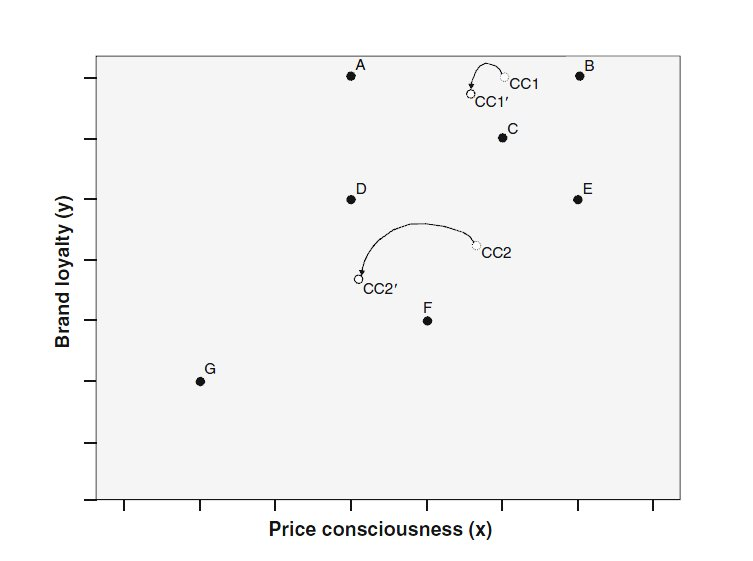
\includegraphics[scale=0.6]{images/kmeans3.jpg}\\
 	\end{center}
 \end{figure}
 \begin{figure}[h!]
\begin{center}
 		% Requires \usepackage{graphicx}
 		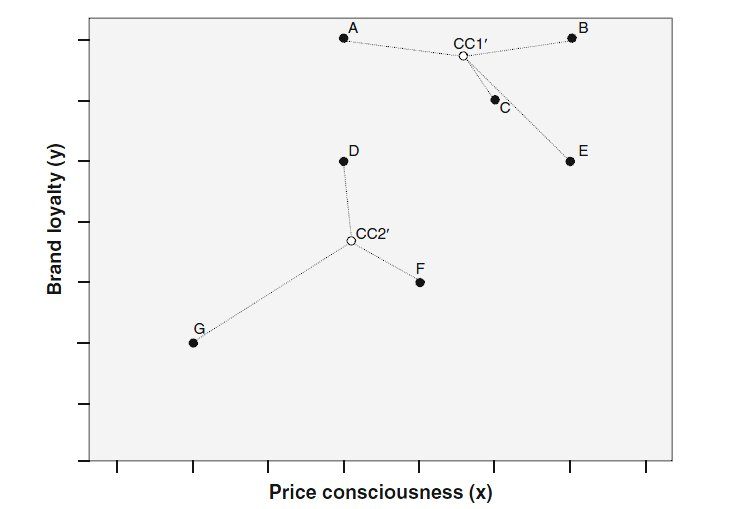
\includegraphics[scale=0.6]{images/kmeans4.jpg}\\
 	\end{center}
 \end{figure}
 Both clusters�centers now shift into new positions (CC1� for the first and CC2� for the second cluster).
 In the fourth step, the distances from each object to the newly located cluster
 centers are computed and objects are again assigned to a certain cluster on the basis
 of their minimum distance to other cluster centers (CC1� and CC2�).
 
 Since the cluster centers� position changed with respect to the initial situation in the first step,
 this could lead to a different cluster solution. This is also true of our example, as
 object E is now � unlike in the initial partition � closer to the first cluster center
 (CC1�) than to the second (CC2�). Consequently, this object is now assigned to the
 first cluster.
 The k-means procedure now repeats the third step and
 re-computes the cluster centers of the newly formed clusters, and so on.
 In other words, steps 3 and 4 are repeated until a predetermined number of iterations are
 reached, or convergence is achieved (i.e., there is no change in the cluster affiliations).
 
\subsection{Optimal Number of Clusters}
One of the biggest problems with cluster analysis is identifying the optimum number of
clusters. As the joining process continues, increasingly dissimilar clusters must be joined. i.e. the classification becomes increasingly artificial. Deciding upon the optimum number
of clusters is largely subjective, although looking at a dendrogram would help.

\subsection{Optimal Number of Clusters}
One of the biggest problems with cluster analysis is identifying the optimum number of
clusters. As the joining process continues, increasingly dissimilar clusters must be joined. i.e. the classification becomes increasingly artificial. Deciding upon the optimum number
of clusters is largely subjective, although looking at a dendrogram would help.

% http://www.uk.sagepub.com/burns/data.htm
% Data Set 23 A

% DASL
% http://lib.stat.cmu.edu/cgi-bin/dasl.cgi?query=Cluster+analysis&submit=Search%21&metaname=methods&sort=swishrank



% http://www.uk.sagepub.com/burns/website%20material/Chapter%2023%20-%20Cluster%20Analysis.pdf
% http://www.cs.uu.nl/docs/vakken/arm/additional/additional.html
% Cluster Analysis :  http://www.cs.uu.nl/docs/vakken/arm/SPSS/spss8.pdf
% Discriminant Analaysis : http://www.cs.uu.nl/docs/vakken/arm/SPSS/spss6.pdf
% Factor Analysis : http://www.cs.uu.nl/docs/vakken/arm/SPSS/spss7.pdf




The hierarchical clustering procedure attempts to identify relatively homogeneous groups of cases (or variables) based on selected
characteristics. For example: cluster television shows into homogeneous groups based on viewer
characteristics. In hierarchical clustering, an algorithm is used that starts with each case (or variable) in a
separate cluster and combines clusters until only one is left.



To cluster cases you need to identify variables you wish to be considered in creating clusters for the cases.
The variables to be used for cluster formation are here: picture quality (5 measures), reception quality (3
measures), audio quality (3 measures), ease of programming (1 measure), number of events (1 measure),
number of days for future programming (1 measure), remote control (3 measures), and extras (3 measures).
Pass these in the Variable(s) box.

Cluster Method: Choose the procedure for combining clusters. The default procedure is called the
between-group linkage. SPSS computes the smallest average distance between all group pairs and
combines the two groups that are closest. The procedure begins with as many clusters as there are cases
(here: 21). At step one, the two cases with the smallest distance between them are clustered. Then SPSS
computes distances once more and combines the two that are next closest. After the second step you will
have either 18 individual cases and one cluster of 3 cases, or 17 individual cases and two clusters of two
cases each. The process continues until all cases are grouped into one large cluster.
Measure: Indicate what method is used for distance measuring, the default is Squared Euclidean distance. 




 \subsection{Performance of k-means clustering}
 Generally, k-means is superior to hierarchical methods as it is less affected by
 outliers and the presence of irrelevant clustering variables. Furthermore, k-means
 can be applied to very large data sets, as the procedure is less computationally
 demanding than hierarchical methods. In fact, we suggest definitely using k-means
 for sample sizes above 500, especially if many clustering variables are used. From
 a strictly statistical viewpoint, k-means should only be used on interval or ratio-scaled
 data as the procedure relies on Euclidean distances. However, the procedure is
 routinely used on ordinal data as well, even though there might be some distortions.
 
 One problem associated with the application of k-means relates to the fact that
 the researcher has to pre-specify the number of clusters to retain from the data. This
 makes k-means less attractive to some and still hinders its routine application in
 practice.

%------------------------------------------------------------------%
\newpage


%------------------------------------------------------------------%
\newpage

\section{Important Considerations for Two-Step Clustering}

\section{Two-Step Cluster}

The Two-Step Cluster Analysis procedure was designed for such applications. The name two-step clustering is already an indication that the algorithm is based on a two-stage approach: In the first stage, the algorithm undertakes a procedure that is very similar to the k-means algorithm. 

Based on these results, the two-step
procedure conducts a modified hierarchical agglomerative clustering procedure that
combines the objects sequentially to form homogenous clusters. This is done by
building a so-called \textbf{\textit{cluster feature tree}} whose \textbf{\textit{leaves}} represent distinct objects in the dataset. 

The procedure can handle categorical and continuous variables simultaneously
and offers the user the flexibility to specify the cluster numbers as well as
the maximum number of clusters, or to allow the technique to automatically choose
the number of clusters on the basis of statistical evaluation criteria.

\subsection{Cluster Features Tree}

Two-Step Cluster Analysis is done by building a so-called \textbf{\textit{cluster feature tree}} whose \textbf{\textit{leaves}} represent distinct objects in the dataset. The procedure can handle categorical and continuous variables simultaneously and offers the user the flexibility to specify the cluster numbers as well as the maximum number of clusters, or to allow the technique to automatically choose the number of clusters on the basis of statistical evaluation criteria.

Additionally, the procedure indicates each variable�s importance for the construction of a specific cluster. These desirable features make the somewhat less popular two-step clustering a viable alternative to the traditional
methods.


\subsection{Types of Data} The Two-Step procedure works with both continuous and categorical variables. Cases represent objects to be clustered, and the variables represent attributes upon which the clustering is based.

\subsection{Case Order}
Note that the cluster features tree and the final solution may depend on the order of objects (or cases). To minimize order effects, randomly order the cases. It is recommended to obtain several different solutions with cases sorted in different random orders to verify the stability of a given solution. In situations where this is difficult due to extremely large file sizes, multiple runs with a sample of cases sorted in different random orders might be substituted.
%------------------------------------------------------------------------------%


\subsection{Graphical Outputs}
The lower part of the output indicates the quality of the cluster
solution. The silhouette measure of cohesion and separation is a measure of the
clustering solution�s overall goodness-of-fit. It is essentially based on the average
distances between the objects and can vary between -1 and +1. Specifically, a
silhouette measure of less than 0.20 indicates a poor solution quality, a measure
between 0.20 and 0.50 a fair solution, whereas values of more than 0.50 indicate a
good solution . In our case, the measure indicates a satisfactory (``fair") cluster quality. Consequently, you can
proceed with the analysis by double-clicking on the output. This will open up the
model viewer , an evaluation tool that graphically presents the structure
of the revealed clusters.


The model viewer provides us with two windows: the main view, which initially
shows a model summary (left-hand side), and an auxiliary view, which initially
features the cluster sizes (right-hand side). At the bottom of each window, you can
request different information, such as an overview of the cluster structure and the
overall variable importance.
%------------------------------------------------------------------------------%





\section{Two-Step Cluster Analysis}

When you have a really large data set or you need a clustering procedure that can rapidly form clusters on the basis of either categorical or continuous data, neither of the previous two procedures are entirely appropriate. Hierarchical clustering requires a matrix of distances between all pairs of cases, and k-means requires shuffling cases in and out of clusters and knowing the number of clusters in advance.

The Two-Step Cluster Analysis procedure was designed for such applications. The name two-step clustering is already an indication that the algorithm is based on a two-stage approach
\begin{itemize}
	\item In the first stage, the algorithm undertakes a procedure that is very similar to the k-means algorithm. \item Based on these results, the two-step
	procedure conducts a modified hierarchical agglomerative clustering procedure that
	combines the objects sequentially to form homogenous clusters.
\end{itemize}

The Two-Step Cluster Analysis is an exploratory tool designed to reveal natural groupings (or clusters) within a data set that would otherwise not be apparent. The algorithm employed by this procedure has several desirable features that differentiate it from traditional clustering techniques:

\begin{itemize}
	\item Handling of categorical and continuous variables. By assuming variables to be independent, a joint \textbf{\textit{multinomial-normal distribution}} can be placed on categorical and continuous variables. (Interesting, but not examinable).
	
	\item Automatic selection of number of clusters. By comparing the values of a \textbf{\textit{model-choice criterion}} across different clustering solutions, the procedure can automatically determine the optimal number of clusters.
	
	\item Scalability. By constructing a \textbf{\textit{cluster features}} (CF) tree that summarizes the records, the Two-Step algorithm allows you to analyze large data files. The Two-Step Cluster Analysis requires only one pass of data (which is important for very large data files).
	
\end{itemize}
The Two-Step Cluster Analysis requires only one pass of data
(which is important for very large data files).

Additionally, the procedure indicates each variable�s
importance for the construction of a specific cluster. These desirable features make
the somewhat less popular two-step clustering a viable alternative to the traditional
methods.


\subsection{Pre-clustering }

In two-step clustering, to make large problems tractable, in the first step, cases are
assigned to \textbf{\textit{preclusters}}. In the second step, the preclusters are clustered using the
hierarchical clustering algorithm. You can specify the number of clusters you want or
let the algorithm decide based on preselected criteria.

In general, the larger the number of sub-clusters produced by the pre-cluster step, the more accurate the final result is. However, too many sub-clusters will slow down the clustering during the second step.

The maximum number of sub-clusters should be carefully chosen so that it is large enough to produce accurate results and small enough not to slow down the second step clustering.






%----------------------------------------------------------------------%
\subsection{Measures of Fit}
Two-Step Cluster Analysis guides the decision of how many clusters to retain from the data by
calculating measures-of-fit such as \textbf{\textit{Akaike�s Information Criterion (AIC)}} or \textbf{\textit{Bayes Information Criterion (BIC)}}.

These are relative measures of goodness-of-fit and are used to compare different
solutions with different numbers of segments.(``Relative" means that these criteria
are not scaled on a range of, for example, 0 to 1 but can generally take any value.)
Compared to an alternative solution with a different number of segments, smaller
values in AIC or BIC indicate an increased fit.

SPSS computes solutions for different
segment numbers (up to the maximum number of segments specified before) and
chooses the appropriate solution by looking for the smallest value in the chosen
criterion. However, which criterion should we choose? AIC is well-known for
overestimating the correct number of segments, while BIC has a slight tendency
to underestimate this number.

Thus, it is worthwhile comparing the clustering
outcomes of both criteria and selecting a smaller number of segments than
actually indicated by AIC. Nevertheless, when running two separate analyses,
one based on AIC and the other based on BIC, SPSS usually renders the same
results.
\newpage


The clustering algorithm is based on a distance measure that gives the best results if all variables are independent, continuous variables have a normal distribution (or categorical variables have a multinomial distribution). This is seldom the case in practice, but the algorithm is thought to behave reasonably well when the assumptions are not met.

Because cluster analysis does not involve hypothesis testing and calculation of observed significance levels, other than for descriptive follow-up, it's perfectly acceptable to cluster data that may not meet the assumptions for best performance.

The final outcome may depend on the order of the cases in the file. To minimize the effect, arrange the cases in random order. Sort them by the last digit of their ID numbers or something similar.

\subsection{Step 1 : Pre-clustering: Making Little Clusters}
The first step of the two-step procedure is formation of pre-clusters. The goal of pre-clustering is to reduce the size of the Distance matrix (the matrix that contains distances between all
possible pairs of cases). Pre-clusters are just clusters of the original cases that are used in place of the raw data in the hierarchical clustering. As a case is read, the algorithm
decides, based on a distance measure, if the current case should be merged with a previously formed pre-cluster or start a new precluster.

When preclustering is complete, all cases in the same precluster are treated as a single entity. The size of the distance matrix is no longer dependent on the number of cases but on the number of preclusters.



\subsection{Step 2 : Hierarchical Clustering of Preclusters}
In the second step, SPSS uses the standard hierarchical clustering algorithm on the
preclusters. Forming clusters hierarchically lets you explore a range of solutions with
different numbers of clusters.
Tip: The Options dialog box lets you control the number of preclusters. Large numbers
of preclusters give better results because the cases are more similar in a precluster;
however, forming many preclusters slows the algorithm.


Some of the options you can specify when using two-step clustering are:
\textbf{Standardization:} The algorithm will automatically standardize all of the variables
unless you override this option.

\textbf{Distance measures:} If your data are a mixture of continuous and categorical variables,
you can use only the log-likelihood criterion. The distance between two clusters
depends on the decrease in the log-likelihood when they are combined into a single
cluster. If the data are only continuous variables, you can use the Euclidean
distance between two cluster centers. Depending on the distance measure selected,
cases are assigned to the cluster that leads to the largest log-likelihood or to the cluster
that has the smallest Euclidean distance.


\textbf{Number of clusters:} You can specify the number of clusters to be formed, or you can let
the algorithm select the optimal number based on either the Schwarz Bayesian
Criterion or the Akaike information criterion.


\textbf{Outlier handling:} You have the option to create a separate cluster for cases that don't fit
well into any other cluster.


\textbf{Range of solutions:} You can specify the range of cluster solutions that you want to see.

\subsection{SPSS Implementation}

\begin{itemize}
	\item To implement a Two-Step Cluster Analysis in SPSS, you use the following options:\\
	\textbf{\textit{Analyze $>$ Classify $>$ TwoStep Cluster}}.
	
	\item \textbf{Distance Measure} Log likelihood distance measures are the default; Euclidean distance can be used if all variables are continuous. (Log likelihood distance measures are not part of course).
	
	\item \textbf{Count of Continuous Variables} Continuous variables are standardized by default. The variables
	are standardized so that they all contribute equally to the distance or similarity between cases.
	
	\item \textbf{Number of clusters} You can specify the number of clusters, or you can let the algorithm select
	the optimal number based on either the Schwarz Bayesian criterion (BIC) or the Akaike
	information criterion (AIC).
	
	\item \textbf{Clustering Criterion} BIC and AIC are offered with the default being BIC.
\end{itemize}




\end{document}